\section{Introduction}

Powder X-ray diffraction (PXRD) is the most widely available probe for characterizing crystalline intermediates, yet turning a noisy one-dimensional scattering profile into an atomic structure still hinges on manual Rietveld-style refinement, curated priors, and hours of expert iteration~\cite{toby2013gsas2,rodriguezcarvajal1993fullprof,Cheetham2014}. Fully autonomous PXRD workflows therefore require models that can translate raw intensities into crystallographic information files (CIFs) while remaining faithful to experimental noise and instrument effects.

Autoregressive language models conditioned on PXRD embeddings (\eg, \deCIFer~\cite{deCIFer2025}) have taken important steps in this direction by directly generating CIF tokens from diffraction traces. However, the baseline exposed three systemic bottlenecks: (i) multi-day training due to inefficient data serving and augmentation, (ii) a single decoding rule that selects candidates solely by language-model likelihood, without a separate PXRD-based scoring step, and (iii) ad hoc evaluation of candidate CIF portfolios when chemical composition or symmetry descriptors are missing.

We introduce \xtoCIF, a practitioner-oriented extension that revisits training, decoding, and evaluation for PXRD-to-structure models. The framework accelerates data loading and PXRD augmentation, exposes scriptable deterministic beam search alongside the default stochastic sampler, and provides utilities that order candidate CIFs by their post hoc weighted-profile residual (\(\Rwp\)). Collectively, these changes enable systematic comparison across descriptor‑free, composition-conditioned, and composition‑plus‑space‑group regimes without altering the underlying autoregressive architecture or tokenizer.

On the NOMA benchmark, the proposed training stack delivers \(\sim44\times\) higher throughput while maintaining fidelity to experimental artifacts, and the decoding protocol improves both match rate (MR) and \(\Rwp\) in low-information settings. For comparability, we retain the MR, validity, and \(\Rwp\) metrics established by \deCIFer and report all ablations in the same evaluation harness.


\paragraph{Contributions.} Relative to \deCIFer, \xtoCIF keeps the autoregressive generator and tokenizer unchanged. We contribute three self-contained, quantified components:
\begin{itemize}
  \item \textbf{Training system (engineering).} A GPU-optimized pipeline that delivers \(\sim\!44\times\) higher throughput on NOMA via streamlined data serving, efficient PXRD augmentation, and multi-GPU orchestration. Single-GPU iteration time drops from \(257.9\!\pm\!4.2\) s to \(10.35\!\pm\!0.13\) s, and to \(5.82\!\pm\!0.19\) s on 2 GPUs (\(124\!\pm\!2\) and \(220\!\pm\!7\) samples/s respectively), reducing wall-clock training time by roughly \(44\times\) for a fixed step budget (Table~\ref{tab:train-optimization-throughput}). This acceleration allowed us to sweep dozens of random seeds and initialization strategies, raising the composition-conditioned MR to \(\approx97\%\) without modifying the \deCIFer backbone (Table~\ref{tab:decoding_refinements}); the original \deCIFer report lists \(\approx94\%\) for this regime~\cite{deCIFer2025}.
  \item \textbf{Inference protocol.} We expose deterministic beam search alongside the stochastic sampler and make it easy to sweep beam widths through the shared evaluation harness. Candidates are subsequently ordered by their computed \(\Rwp\) using the same utilities, which enables post hoc filtering of the beam without modifying checkpoints. In the descriptor‑free regime on NOMA this workflow reduces \(\Rwp\) from 0.23 to 0.18 and raises match rate (MR) from 5.6\% to 8.1\% (\(+45\%\) relative); with Comp or Comp+SG, \xtoCIF keeps MR near 97.3\% while trimming \(\Rwp\) by \(\sim0.03\) (Tab.~\ref{tab:decoding_refinements}).
  \item \textbf{Evaluation protocol.} A unified, reproducible protocol across three conditioning regimes (\emph{No descriptors} / \emph{Comp} / \emph{Comp+SG}) with standardized metrics: \emph{Validity} (syntax/unit-cell parameters/bond sanity), \emph{MR} (RMSD \(\le 0.5\,\text{\AA}\) after symmetry-aware alignment that enforces chemical identity), and \(\Rwp\) computed on simulated PXRD. Unless stated otherwise, we report aggregated statistics over generated candidates (best-of-beam extracted via the post hoc filtering stage plus global medians/means). Fig.~\ref{fig:beam_rmsd_match} shows how these aggregates evolve with beam size.
\end{itemize}

% !TeX root = ../cvpr_main.tex
% Figure 1: XtoCIF overview (TikZ)
% Use [H] to prevent the figure from floating
% above the preceding paragraph (requires \usepackage{float} in the preamble).
\newcommand{\diffractogramIcon}{%
  % Fit within node width and crop out the bitmap title (keep axes only)
  % trim = left bottom right top
  \includegraphics[width=0.98\linewidth,clip,trim=0pt 0pt 0pt 28pt]{Figures/illustrations/xtocif_pxrd_input.png}%
}
\newcommand{\augmentIllustration}{%
  % Enlarge the augmentation example and crop outer whitespace
  \includegraphics[width=0.98\linewidth,clip,trim=6pt 6pt 6pt 10pt]{Figures/data_statistics/noisebroadness}%
}
% Encoder icon: use provided SVG artwork instead of the TikZ placeholder
% Source: Figures/illustrations/encoder_neural_network.svg
\newcommand{\encoderIcon}{%
  % Prefer pre-converted PDF for portability; fallback to SVG if needed
  \IfFileExists{Figures/illustrations/encoder_neural_network.pdf}{%
    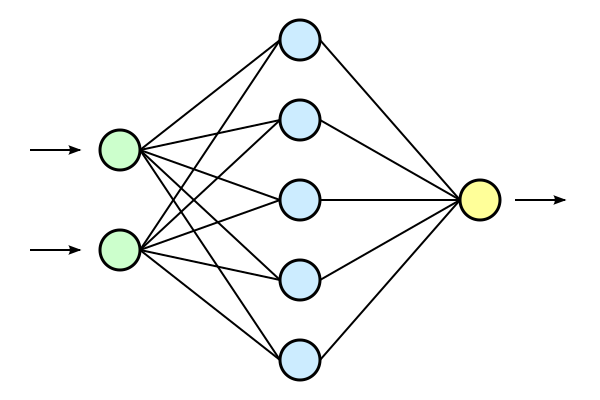
\includegraphics[width=0.98\linewidth]{Figures/illustrations/encoder_neural_network.pdf}%
  }{%
    % Requires: \usepackage{svg} in the preamble
    \includesvg[width=0.98\linewidth]{Figures/illustrations/encoder_neural_network}%
  }%
}
% --- Decoder icon: clean arrow only (sized for small block) -------------------
\newcommand{\decoderIcon}{%
  % Minimal but informative: Tokens → Decoder ×N → Logits
  \resizebox{\linewidth}{!}{%
    \begin{tikzpicture}[
      name prefix=decicon-,
      baseline=(current bounding box.center),
      >=Latex,
      % Ensure text inside the mini icon stays ≥7 pt
      node/.style={rounded corners=2pt, draw=black, line width=0.6pt, fill=white, minimum height=5mm, inner sep=2pt, font=\scriptsize}
    ]
      \node[node, minimum width=10mm] (tok) {Tokens};
      \node[node, minimum width=16mm, right=0.22cm of tok] (dec) {Decoder $\times N$};
      \node[node, minimum width=10mm, right=0.22cm of dec] (log) {Logits};
      \draw[-{Latex[length=2.6pt,width=2.3pt]}, line width=0.7pt] (tok.east) -- (dec.west);
      \draw[-{Latex[length=2.6pt,width=2.3pt]}, line width=0.7pt] (dec.east) -- (log.west);
    \end{tikzpicture}%
  }%
}
% Crystal structure + PXRD mini icon for simulation panel
\newcommand{\crystalPxrdIcon}{%
  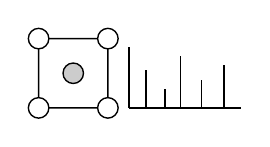
\begin{tikzpicture}[
    x=0.22cm, y=0.22cm,
    baseline=(current bounding box.center),
    atom/.style={circle, draw=black, fill=white, line width=0.5pt, inner sep=0pt, minimum size=2.6mm},
    axis/.style={line width=0.6pt}
  ]
    % Unit cell (simple square + lattice points)
    \begin{scope}[shift={(0,0)}]
      \draw[line width=0.6pt, rounded corners=1pt] (0,0) rectangle (4,4);
      \node[atom] at (0,0)    {};
      \node[atom] at (4,0)    {};
      \node[atom] at (0,4)    {};
      \node[atom] at (4,4)    {};
      \node[atom, fill=black!20] at (2,2) {};
    \end{scope}
    % Mini PXRD to the right
    \begin{scope}[shift={(5.2,0)}]
      % axes
      \draw[axis] (0,0) -- (6.5,0);
      \draw[axis] (0,0) -- (0,3.5);
      % a few peaks
      \draw[line width=0.6pt] (1.0,0) -- (1.0,2.2);
      \draw[line width=0.6pt] (2.1,0) -- (2.1,1.1);
      \draw[line width=0.6pt] (3.0,0) -- (3.0,3.0);
      \draw[line width=0.6pt] (4.2,0) -- (4.2,1.6);
      \draw[line width=0.6pt] (5.5,0) -- (5.5,2.5);
    \end{scope}
  \end{tikzpicture}%
}
% Panel for Simulate PXRD: use dataset-based image and overlay arrow (structure → PXRD)
\newcommand{\simulatePxrdPanel}{%
  % Ensure the composite panel always fits the enclosing node width
  \resizebox{\linewidth}{!}{%
    \begin{tikzpicture}[name prefix=sim-, baseline=(current bounding box.center)]
      \node[inner sep=0pt] (stru) {\includegraphics[width=0.52\linewidth]{Figures/illustrations/simulate_pxrd_ds_structure.png}};
      \node[inner sep=0pt, below=0.22cm of stru] (pxrd) {\includegraphics[width=0.74\linewidth]{Figures/illustrations/simulate_pxrd_ds_pxrd.png}};
      % Arrow starts just below structure and ends just above PXRD
      \draw[-{Latex[length=4pt,width=3.4pt]}, line width=1.0pt]
        ($(stru.south)+(0,-0.02)$) -- ($(pxrd.north)+(0,0.02)$);
    \end{tikzpicture}%
  }%
}
% Beam-search illustration sourced from the final frame of Beam\_search.gif (Wikimedia Commons)
\newcommand{\beamTreeIcon}{%
  % Crop away the black border from the source PNG
  \includegraphics[width=0.7\linewidth,clip,trim=3pt 3pt 3pt 3pt]{Figures/illustrations/beam_search_last.png}%
}
\newcommand{\rwpRankingIllustration}{%
  \includegraphics[width=0.92\linewidth]{Figures/illustrations/rwp_ranking_pxrd.png}%
}
% High-contrast fills (avoid low-contrast pastels)
\colorlet{xtoinput}{white}
\colorlet{xtomodel}{white}
\colorlet{xtodecode}{white}
\colorlet{xtoeval}{white}
% Daltonian-safe palette (Okabe–Ito)
\definecolor{oiBlue}{HTML}{0072B2}          % inherited → blue (dashed)
\definecolor{cbRed}{HTML}{E41A1C}           % contributions → true red (ColorBrewer Set1)
\colorlet{deciferOutline}{oiBlue}
\colorlet{xtocifContributionOutline}{cbRed}
\begingroup
% Tighten vertical white space around the float for CVPR columns
\setlength{\textfloatsep}{3pt plus 1pt minus 1pt}
\setlength{\intextsep}{3pt plus 1pt minus 1pt}
\begin{figure}[t]
  \centering
  % Keep within column bounds with comfortable margins under CVPR review rulers
  \begin{adjustbox}{center,max width=0.80\linewidth}
  \begin{tikzpicture}[
    >=Latex,
    % Zero outer sep so connectors touch the drawn border exactly
    % Use ≥\footnotesize everywhere for readability at 1-col scale
    block/.style={draw, rounded corners=4pt, align=center, text=black, font=\footnotesize, line width=1.0pt, inner sep=3pt, minimum height=8mm, outer sep=0pt},
    inputBlock/.style={block, fill=white},
    modelBlock/.style={block, fill=white},
    decodeBlock/.style={block, fill=white},
    evalBlock/.style={block, fill=white},
    % Connectors: main path (solid) and optional deps (dashed)
    connectorMain/.style={-{Latex[length=3pt,width=2.5pt]}, line width=0.95pt, shorten >=1.2pt, shorten <=1.2pt, line cap=round},
    connectorOpt/.style={connectorMain, dashed},
    legendBox/.style={rectangle, rounded corners=2pt, minimum width=0.5cm, minimum height=0.28cm},
    legendDot/.style={circle, minimum size=0.3cm, inner sep=0pt}
  ]
    % Unified block width
    \newlength{\xtocifBlockWidth}
    % Enlarge blocks slightly while keeping within column bounds
    \setlength{\xtocifBlockWidth}{31mm}% single source of truth
    \matrix (flow) [
      row sep=0.90cm,
      column sep=0.50cm
    ]{
      \node[inputBlock, draw=deciferOutline, dashed, text width=\xtocifBlockWidth] (pxrdIn) {\diffractogramIcon\\[1pt]\textbf{PXRD Trace $(2\theta, I)$}}; &
      \node[inputBlock, draw=deciferOutline, dashed, text width=\xtocifBlockWidth] (aug) {\textbf{Augment \& Normalize}\\[1pt]\augmentIllustration}; &
      \node[modelBlock, draw=deciferOutline, dashed, text width=\xtocifBlockWidth] (enc) {\textbf{PXRD Encoder}\\1D CNN + Transformer\\[2pt]\encoderIcon}; \\
      \node[modelBlock, draw=deciferOutline, dashed, text width=\xtocifBlockWidth] (desc) {\textbf{Descriptors $\oplus$}\\None / Comp / Comp+SG}; &
      \node[modelBlock, draw=deciferOutline, dashed, text width=\xtocifBlockWidth] (cond) {\textbf{Conditioning}}; &
      \node[modelBlock, draw=deciferOutline, dashed, text width=\xtocifBlockWidth] (decBlock) {\textbf{Decoder (AR)}\\[1pt]\decoderIcon}; \\
      \node[evalBlock, draw=xtocifContributionOutline, text width=\xtocifBlockWidth] (rwp) {\textbf{Rwp Reranking}\\[-2pt]\rwpRankingIllustration}; &
      \node[evalBlock, draw=xtocifContributionOutline, text width=\xtocifBlockWidth] (sim) {\textbf{Simulate PXRD}\\\footnotesize Per CIF\\[1pt]\simulatePxrdPanel}; &
      \node[evalBlock, draw=xtocifContributionOutline, text width=\xtocifBlockWidth] (beam) {\textbf{Beam Search}\\[1pt]\beamTreeIcon}; \\
      \node[coordinate] (gapL) {}; &
      \node[evalBlock, draw=xtocifContributionOutline, text width=\xtocifBlockWidth] (out) {\textbf{Top-k CIFs}}; &
      \node[coordinate] (gapR) {}; \\
    };

    % Flow edges (solid = main path, dashed = optional dependency)
    \draw[connectorMain] (pxrdIn) -- (aug);
    \draw[connectorMain] (aug) -- (enc);
    \draw[connectorMain] (enc) -- (cond);
    \draw[connectorOpt] (desc.east) -- (cond.west);
    % (Optional) descriptors indicated in-block via $\oplus$ symbol
    \draw[connectorMain] (cond) -- (decBlock);
    % Centered vertical link decoder → beam
    \draw[connectorMain] (decBlock.south) -- (beam.north);
    \draw[connectorMain] (beam) -- (sim);
    \draw[connectorMain] (sim) -- (rwp);
    \draw[connectorMain] (rwp.south) |- (out);

    % (Removed stage label previously reading: "PXRD observation & conditioning")

    % Compact legend: two colored pastilles (dashed = inherited, solid = contributions)
    % Compact legend placed to the right of Top-K block
    \matrix (legend) [
      font=\scriptsize,
      column sep=2mm,
      row sep=0.5mm,
      anchor=west
    ] at ($(out.east)+(0.25cm,0)$) {
      \node[legendDot, draw=deciferOutline, dashed, fill=white, line width=1.0pt] {}; &
      \node[text=deciferOutline, font=\scriptsize\bfseries] {Inherited from \deCIFer}; \\
      \node[legendDot, draw=xtocifContributionOutline, fill=white, line width=1.0pt] {}; &
      \node[text=xtocifContributionOutline, font=\scriptsize\bfseries] {Contributions}; \\
      % Optional legend row removed
    };
    % No explanatory sentence to keep the legend compact
  \end{tikzpicture}
  \end{adjustbox}
  \caption{\xtoCIF pipeline: PXRD $\rightarrow$ encoder (+descriptors) $\rightarrow$ decoder $\rightarrow$ beam search $\rightarrow$ PXRD simulation $\rightarrow$ $\Rwp$ reranking $\rightarrow$ Top-$k$; \textcolor{deciferOutline}{blue dashed} = inherited, \textcolor{xtocifContributionOutline}{red solid} = contributions.}
  \label{fig:xtocif_overview}
  % Trim a bit of space below the caption in review mode
  \vspace{-6pt}
\end{figure}
\endgroup

